%http://www.daniel-brettschneider.de/allgemein/latex-vorlage-fur-hausarbeiten-oder-abschlussarbeiten
\documentclass[12pt,a4paper,bibliography=totocnumbered,listof=totocnumbered, abstracton]{scrartcl}

\usepackage[autostyle=true,german=quotes]{csquotes}
\usepackage[utf8]{inputenc}
\usepackage{amsmath}
\usepackage{amsfonts}
\usepackage{amssymb}
\usepackage{amsthm}
\usepackage{graphicx}
\usepackage{fancyhdr}
\usepackage{tabularx}
\usepackage{geometry}
\usepackage{setspace}
\usepackage[right]{eurosym}
\usepackage[printonlyused]{acronym}
\usepackage{subfig}
\usepackage{floatflt}
\usepackage[usenames,dvipsnames]{color}
\usepackage{colortbl}
\usepackage{paralist}
\usepackage{array}
\usepackage{titlesec}
\usepackage{parskip}
\usepackage[right]{eurosym}
\usepackage[subfigure,titles]{tocloft}
\usepackage[pdfpagelabels=true]{hyperref}
\usepackage[ngerman]{babel}
\usepackage{booktabs}
\usepackage{listings}
\usepackage{csquotes}
\usepackage{siunitx}
\newtheoremstyle{Umgebung}	% name
{20pt}	% Space above, empty = `usual value'
{20pt} % Space below
{} % Body font
{} % Indent amount (empty = no indent, \parindent = para indent)
{\bfseries} % Thm head font
{} % Punctuation after thm head
{\newline} % Space after thm head: \newline = linebreak
{} % Thm head spec


\theoremstyle{Umgebung}

\lstset{basicstyle=\footnotesize, captionpos=b, breaklines=true, showstringspaces=false, tabsize=2, frame=lines, numbers=left, numberstyle=\tiny, xleftmargin=2em, framexleftmargin=2em}
\makeatletter
\def\l@lstlisting#1#2{\@dottedtocline{1}{0em}{1em}{\hspace{1,5em} Lst. #1}{#2}}
\makeatother
\geometry{a4paper, top=27mm, left=30mm, right=20mm, bottom=35mm, headsep=10mm, footskip=12mm}
\hypersetup{unicode=false, pdftoolbar=true, pdfmenubar=true, pdffitwindow=false, pdfstartview={FitH},
	pdftitle={Ausarbeitung Projektvortrag Fuzzy-Regelung},
	pdfauthor={Joel Bartelheimer, Nico Müller},
	pdfsubject={Ausarbeitung Fuzzy-Reglung},
	pdfcreator={\LaTeX\ with package \flqq hyperref\frqq},
	pdfproducer={pdfTeX \the\pdftexversion.\pdftexrevision},
	pdfkeywords={Ausarbeitung Projektvortrag Fuzzy-Regelung},
	pdfnewwindow=true,
	colorlinks=true,linkcolor=black,citecolor=black,filecolor=magenta,urlcolor=black}
\pdfinfo{/CreationDate (D:20110620133321)}
\begin{document}
\titlespacing{\section}{0pt}{12pt plus 4pt minus 2pt}{-6pt plus 2pt minus 2pt}
% Kopf- und Fusszeile
\renewcommand{\sectionmark}[1]{\markright{#1}}
\renewcommand{\leftmark}{\rightmark}
\pagestyle{fancy}
\lhead{}
\chead{}
\rhead{\thesection\space\contentsname}
\lfoot{Ausarbeitung Projektvortrag Fuzzy-Regelung}
\cfoot{}
\rfoot{ Seite \thepage}
\renewcommand{\headrulewidth}{0.4pt}
\renewcommand{\footrulewidth}{0.4pt}
% Vorspann
\renewcommand{\thesection}{\Roman{section}}
\renewcommand{\theHsection}{\Roman{section}}
\pagenumbering{roman}
% ----------------------------------------------------------------------------------------------------------
% Titelseite
% ----------------------------------------------------------------------------------------------------------
\thispagestyle{empty}
\begin{center}
	
\includegraphics[width=5cm]{img/thm2.png}\\
	\vspace*{2cm}
	\Large
	\textbf{Fachbereich}\\
	\textbf{Mathematik, Naturwissenschaften und Informatik }\\
	\vspace*{2cm}
			\Huge
	\textbf{Ausarbeitung Projektvortrag Fuzzy-Regelung}\\
	\vspace*{1.5cm}
		\small
		\textbf{Im Rahmen der Veranstaltung:}\\
		\Large
	\textbf{Praktikum Künstliche Intelligenz(CS5330)}\\
	\vspace*{2cm}
	

	\normalsize
	\newcolumntype{x}[1]{>{\raggedleft\arraybackslash\hspace{0pt}}p{#1}}
	\begin{tabular}{x{7.5cm}x{7.5cm}}
		\rule{0mm}{5ex}\textbf{Autoren:} 
		\newline 
		\newline Joel Bartelheimer
		\newline joel.bartelheimer@mni.thm.de
		\newline 
		\newline Nico Müller
		\newline nico.mueller@mni.thm.de
		\newline
		& 
		\rule{0mm}{5ex}\textbf{Eingereicht bei:} 
		\newline
		\newline  Prof. Dr. Wolfgang Henrich
		\newline
		\newline\rule{0mm}{5ex}\textbf{Abgabedatum:} 
		\newline 14.02.2017
		\newline
	\end{tabular} 
\end{center}
\pagebreak

% ----------------------------------------------------------------------------------------------------------
% Verzeichnisse
% ----------------------------------------------------------------------------------------------------------
% TODO Typ vor Nummer
\renewcommand{\cfttabpresnum}{Tab. }
\renewcommand{\cftfigpresnum}{Abb. }
\settowidth{\cfttabnumwidth}{Abb. 10\quad}
\settowidth{\cftfignumwidth}{Abb. 10\quad}
\titlespacing{\section}{0pt}{12pt plus 4pt minus 2pt}{2pt plus 2pt minus 2pt}
\singlespacing
\rhead{INHALTSVERZEICHNIS}
\renewcommand{\contentsname}{II Inhaltsverzeichnis}
\phantomsection
\addcontentsline{toc}{section}{\texorpdfstring{II \hspace{0.35em}Inhaltsverzeichnis}{Inhaltsverzeichnis}}
\addtocounter{section}{1}
\tableofcontents
\pagebreak
\rhead{VERZEICHNISSE}


% ----------------------------------------------------------------------------------------------------------
% Inhalt
% ----------------------------------------------------------------------------------------------------------
% Abstände Überschrift
\titlespacing{\section}{0pt}{12pt plus 4pt minus 2pt}{-6pt plus 2pt minus 2pt}
\titlespacing{\subsection}{0pt}{12pt plus 4pt minus 2pt}{-6pt plus 2pt minus 2pt}
\titlespacing{\subsubsection}{0pt}{12pt plus 4pt minus 2pt}{-6pt plus 2pt minus 2pt}
% Kopfzeile
\renewcommand{\sectionmark}[1]{\markright{#1}}
\renewcommand{\subsectionmark}[1]{}
\renewcommand{\subsubsectionmark}[1]{}
\lhead{Kapitel \thesection}
\rhead{\rightmark}
\onehalfspacing
\renewcommand{\thesection}{\arabic{section}}
\renewcommand{\theHsection}{\arabic{section}}
\setcounter{section}{0}
\pagenumbering{arabic}
\setcounter{page}{1}

\newtheorem{bsp}{Beispiel}
\newtheorem{defnt}{Definition}

% ----------------------------------------------------------------------------------------------------------
% Einleitung
% ----------------------------------------------------------------------------------------------------------

\section{Problemstellung}

In dem Problemszenario verfolgen sich zwei Autos. Das vordere Auto A wird von einem Menschen geregelt. Das Verfolger Auto B soll durch eine Fuzzy-Regelung gesteuert werden und Auto in einem angemessenen Abstand folgen. Auto B kennt lediglich die eigenen Messwert, dh. nicht die Geschwindigkeit des Auto A, sowie die Entfernung zu Auto A.
Auto B und Auto A haben die gleichen physikalischen Eigenschaften. Die Simulation soll den physikalischen Gesetzen folgen, dh. Luftwiderstand, Höchstgeschwindigkeiten und ein insgesamt realistisches Verhalten ist gefordert. 

\begin{figure}
	\centering
	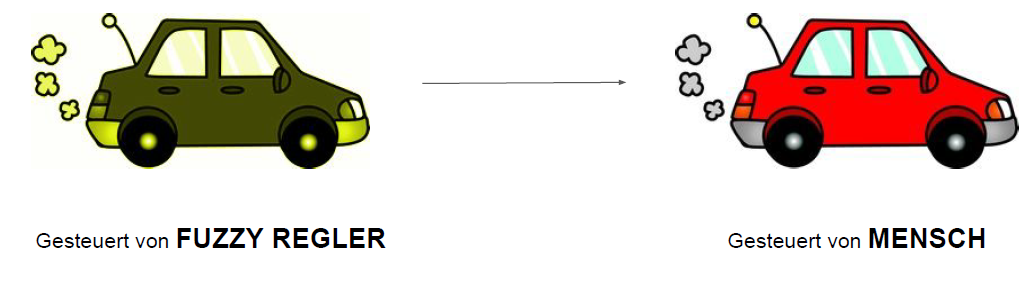
\includegraphics[width=0.9\linewidth]{img/practical/problem}
	\caption{Problemstellung}
	\label{fig:problem}
\end{figure}

\section{GUI}

\begin{figure}
	\centering
	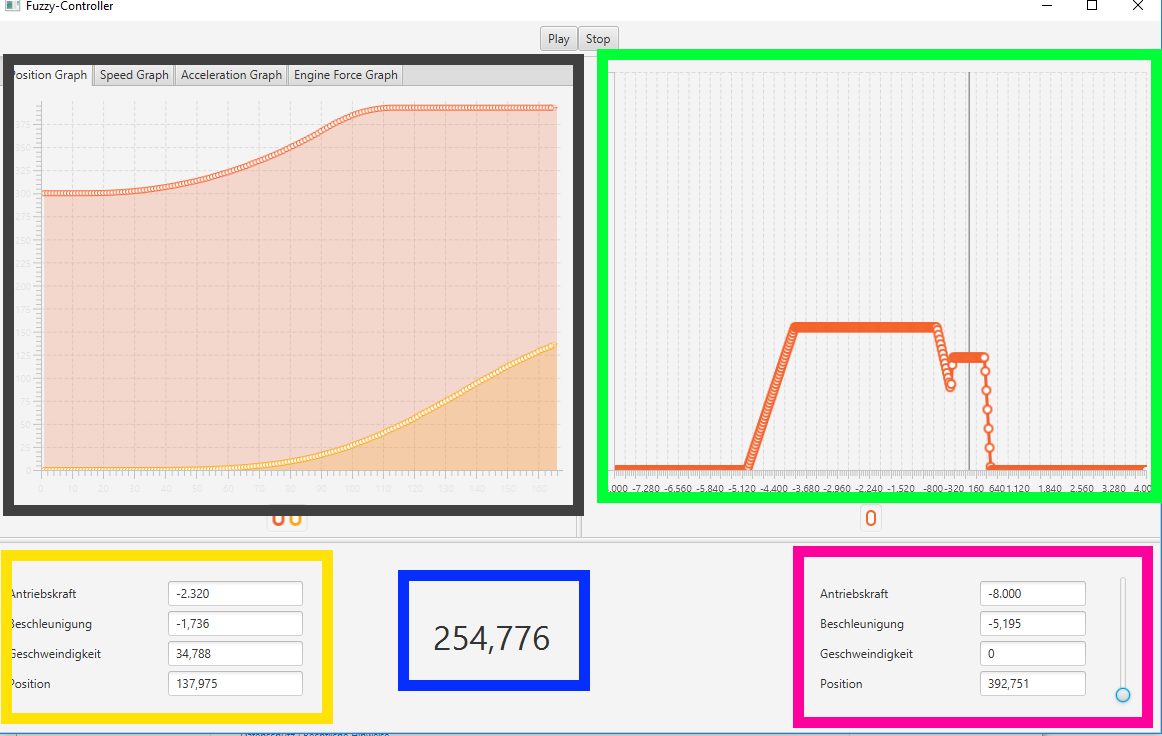
\includegraphics[width=0.9\linewidth]{img/practical/inaction}
	\caption{Die GUI des Regelung-Programs}
	\label{fig:inaction}
\end{figure}

In Abbildung \ref{fig:inaction} ist die GUI des Programms zu sehen. In dem grünen Kasten befindet sich die Ausgangs Fuzzy-Menge die an das Defuzzifizierungsinterface gegeben wird. Die Kästchen Lila und Gelb enthalten jeweils die momentanen Daten von Auto A und B. Für Auto B kann man mit dem Slider die Antriebskraft des vorderen Autos bestimmen. Das blaue Kästchen enthält den momentanen Abstand zwischen den beiden Autos in Metern. Die Tabs in dem schwarzen Kästchen zeigen Echtzeit Informationen über die Simulation. So wird ständig die Position, die Geschwindigkeit, die Beschleunigung und die Antriebskraft geplottet (rot = Auto A und  orange = Auto B).

\section{Konfiguration}

Mögliche Konfigurationen sind:

\begin{itemize}
	\item Partitionierung der Eingangsvariablen
	\item Partitionierung der Ausgangsvariablen
	\item Erstellung der linguistischen Regeln
	\item Wahl der Defuzzifizierungsmethode
\end{itemize}

\begin{figure}
	\centering
	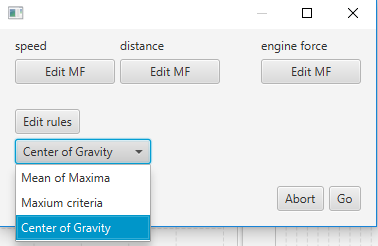
\includegraphics[width=0.7\linewidth]{img/practical/config}
	\caption{Konfugrations Übersicht}
	\label{fig:config}
\end{figure}

\begin{figure}
	\centering
	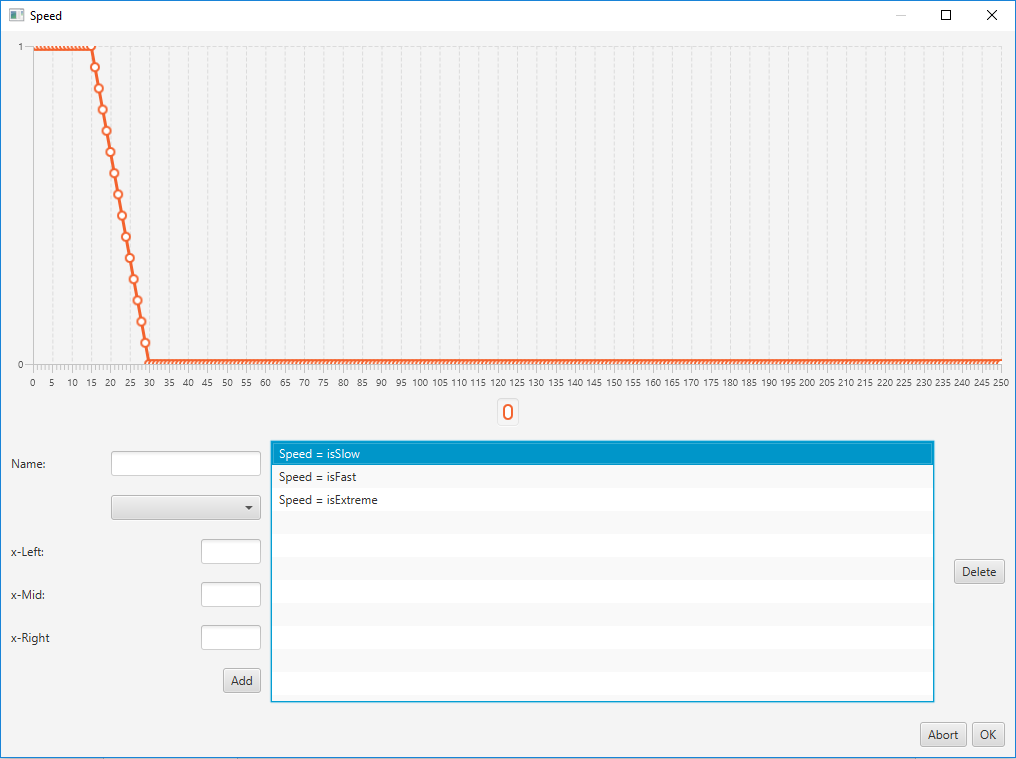
\includegraphics[width=0.7\linewidth]{img/practical/mf}
	\caption{Partitionierung der Fuzzy-Mengen}
	\label{fig:mf}
\end{figure}

\begin{figure}
	\centering
	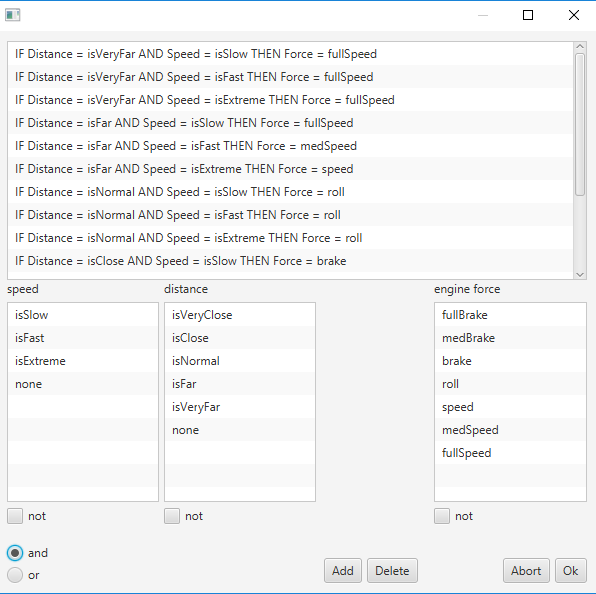
\includegraphics[width=0.7\linewidth]{img/practical/rules}
	\caption{Bestimmung der Linguistischen Regeln}
	\label{fig:rules}
\end{figure}

Es wurden folgende Voreinstellungen für die Regelung gemacht:

\paragraph{Wertebreiche}
Distanz: 0-500 Meter \\
Geschwindigkeit: 0-250 km/h \\
Beschleunigung: -8000-4000 N \\

\paragraph{Partitionierung Distanz}
$\newline$
isVeryClose = $-\infty, 100, 200$ \\
isClose = $100, 200, 300$ \\
isNormal = $250, 300, 350$ \\
isFar = $300, 300, 500$ \\
isVeryFar = $400, 500, \infty$ \\

\paragraph{Partitionierung Geschwindigkeit}
$\newline$
isSlow = $-\infty, 15, 30$ \\
isFast = $15, 50, 100$ \\
isExtreme = $50, 150, 350$ \\

\paragraph{Partitionierung Beschleunigung}
$\newline$
fullBrake = $-\infty, -8000, -7000$ \\
medBrake = $-8000, -5000, -2000$ \\
brake = $-5000, -2000, 0$ \\
roll = $-500, 0, 500$ \\
speed = $0, 1000, 2000$ \\
medSpeed = $1000, 2000, 3000$ \\
fullSpeed = $2000, 3000, \infty$ \\

\paragraph{Regeln}

\begin{lstlisting}
IF Distance = isVeryFar AND Speed = isSlow THEN Force = fullSpeed
IF Distance = isVeryFar AND Speed = isFast THEN Force = fullSpeed
IF Distance = isVeryFar AND Speed = isExtreme THEN Force = fullSpeed
IF Distance = isFar AND Speed = isSlow THEN Force = fullSpeed
IF Distance = isFar AND Speed = isFast THEN Force = medSpeed
IF Distance = isFar AND Speed = isExtreme THEN Force = speed
IF Distance = isNormal AND Speed = isSlow THEN Force = roll
IF Distance = isNormal AND Speed = isFast THEN Force = roll
IF Distance = isNormal AND Speed = isExtreme THEN Force = roll
IF Distance = isClose AND Speed = isSlow THEN Force = brake
IF Distance = isClose AND Speed = isFast THEN Force = medBrake
IF Distance = isClose AND Speed = isExtreme THEN Force = fullBrake
IF Distance = isVeryClose AND Speed = isSlow THEN Force = fullBrake
IF Distance = isVeryClose AND Speed = isFast THEN Force = fullBrake
IF Distance = isVeryClose AND Speed = isExtreme THEN Force = fullBrake

\end{lstlisting}





\section{Implementierung}

Für die Implementierung wird die Sprache \textbf{Scala} verwendet. Folgende Klassen werden verwendet.

\paragraph{Car.scala}

Enthält das physikalische Modell eines Autos.

\paragraph{FuzzyCarController.scala}

Implementierung eines Fuzzy-Controllers nach Mamdami Ansatz.

\paragraph{FuzzyConfig.scala}

Enthält die Klassen: FuzzyTerm.scala, FuzzyRule.scala, FuzzyDefuzzyFunc.scala, FuzzyValueConnector.scala

\paragraph{MembershipFunctions.scala}

Enthält Funktionen wie die Dreiecksfunktion

\section{Probleme}

Leider ist dem Team zu spät aufgefallen, dass es sinnvoll gewesen wäre eine Ableitung des Abstands in die Regelung mit einzubringen. Die gesamte Regelung erscheint nun ein wenig Träge.

% ----------------------------------------------------------------------------------------------------------

\end{document}